\documentclass[a4paper,13pt]{article}
\usepackage[T1]{fontenc}
\usepackage[utf8x]{inputenc}
\usepackage[italian,english]{babel}
\usepackage{amssymb,latexsym,amsfonts,amsmath}
\usepackage{lipsum}
\usepackage{url}
\usepackage{graphicx}
\begin{document}
\author{Andrea Pagliaro , Alessio Susco, Shanj Raul Ken Zaccaretti}
\title{Studio e Progettazione del controllo sulla velocità di rotazione di un generatore eolico}
\maketitle
\section{Introduzione}
\begin{center}
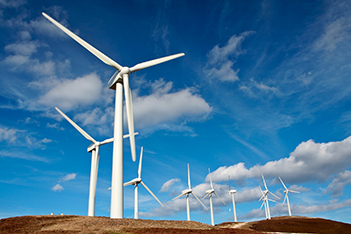
\includegraphics[scale=0.6]{graph/paleoliche.jpg}
\end{center}
Una turbina eolica \'e un dispositivo per estrarre energia dal vento.\\
Tipicamente, il suo rotore \'e progettato in modo da avere tanti gradi di libert\'a
che gli permettano di percepire un flusso del vento tale da ottenere grandi valori potenza.\\
Ovviamente tutto questo deve essere controllato!\\
I controlli fondamentali sono quelli attuati sullo yaw(angolo del rotore rispetto la direzione del vento) e sul pitch , nel seguente testo verr\'a illustrato come funziona quest'ultimo.   
\section{Modello del sistema}
Per far si , che il rotore giri ad una velocit\'a costante in modo che la stessa corrente prodotta non abbia variazioni di frequenza, viene scelto di imporre una giusta angolazione delle pale a seconda della velocit\'a del vento.\\
Gli studi e le ricerche effettuate ci hanno permesso di estrarre equazione di vario genere , ne mostreremo alcune :
\begin{equation}
P=\frac{1}{2}\,\rho\,A\,C_p\,V_w^3
\end{equation}
Che rappresenta la quantit\'a di potenza assorbita dal rotore di una generica turbina eolica presa in considerazione.
Il Cp \'e il coefficiente di potenza , che dipende da $\lambda$ e $\beta$.
Dove a loro volta $\lambda$ \'e dato da :
\begin{equation}
\lambda=\frac{\Omega\,R}{V_w}
\end{equation}
Che viene chiamato tip-speed ratio ed \'e dato dal rapporto tra la velocità angolare
del rotore per il suo raggio e la velocità del vento.
Mentre $\beta$ rappresenta l'angolo di pitch relativo alle pale.
Chiaramente la funzione del coefficiente di potenza comporta delle dinamiche non 
lineari dipendenti dalla geometria del rotore questo a sua volta si ripercuote sull'intero sistema che lo rende non lineare.  
Ora provando a linearizzare il sistema ci \'e risultato molto difficile e solo dopo aver letto alcune pubblicazioni sullo studio di turbine eoliche siamo riusciti a trovare alcune linearizzazioni compiute mediante metodi numerici, che ci hanno permesso di riscrivere il sistema nella seguente forma:
\begin{equation}
\dot{x}=\frac{\gamma}{I_{rot}}x1+\frac{\sigma}{I_{rot}}\,\delta_\beta+\frac{\alpha}{I_{rot}}\,\delta_\omega
\end{equation}
Dove $x$ , lo stato del sistema rappresenta la velocità angolare del rotore ,
$\delta_\beta$ \'e l'ingresso relativo alla perturbazione da parte del pitch,
$\delta_\omega$ \'e la perturbazione relativa alla velocità del vento.
Quindi la nostra matrice di stato \'e data da $A=\frac{\gamma}{I_{rot}}$,
e i coefficienti dei rispettivi ingressi/uscite:
$B=\frac{\sigma}{I_{rot}}$
$\Gamma=\frac{\alpha}{I_{rot}}$
Irot rappresenta inerzia del rotore.
I valori $\gamma$ , $\sigma$ , $\alpha$ rappresentano le derivate parziali ricavate attraverso 
l'equazione dell'aerodinamica del rotore descritta in tal modo:
\begin{equation}
T_{aero}=T(\omega_0,\Omega_0,\beta_0)+\frac{\delta \, T_{aero}}{\delta \, \Omega}+
\frac{\delta \, T_{aero}}{\delta \, \beta}+\frac{\delta \, T_{aero}}{\delta \, \omega}
\end{equation} 
Dove i coefficienti $\gamma=\frac{\delta \, T_{aero}}{\delta \, \Omega}$=-0.1205
$\sigma=\frac{\delta \, T_{aero}}{\delta \, \beta}$=-2.882,
$\alpha=\frac{\delta \, T_{aero}}{\delta \, \omega}$=0.0658
sono gia noti essendo stati ricavati dalla linearizzazione eseguita mediante un metodo numerico non descritto nella pubblicazione di cui si sta facendo uso per il progetto in questione.
I valori degli stati iniziali sono dati da $\omega_0$=18m/s , $\Omega_0$=42RPM e $\beta_0$=12deg.
%----inzio parte controllo nel xaso continuo
\section{Controllo continuo}
Detto questo siamo passati alla progettazione del controllore scegliendo un controllo PI,ovvero proporzionale-intergrativo.\\
Quindi dapprima dobbiamo pensare di avere una retroazione dello stato e
per rendere i calcoli delle costanti pi\'u semplici \'e stato effettuato un cambio di variabile.
\'E stato quindi posto e come l'errore tra l'uscita e il riferimento
\begin{equation*}
	e=x-x_{r}          %--------------------errore---------------------------
\end{equation*}
Voglio che e tenda a 0 per t tendente ad infinito e sapendo che la dinamica dello stato è:
%-----derivata dello stato-----	
\begin{equation*}
	\dot{x}=ax+bu+\gamma w_{d}    %-----------------derivata dello stato------------ 
\end{equation*} \\
Quindi:

\begin{equation*}
	\dot{e}=\dot{x}=a(e+x_{r})+bu+\gamma w_{d}\,\,\:           %-------------spiegazione equazione--------
	\Rightarrow u=u_e-\frac{a}{b} x_{r}-\frac{\gamma}{b} w_{d}
\end{equation*} \\
Dove $u_e$ rappresenter\'a l'errore desiderato che nel nostro caso \'e zero.\\
Volendo attivare un controllo di tipo intergrativo oltre a quello proporzionale
inserisco un ulteriore stao che chiamer\'o $I_e$.\\
A questo punto ottengo un sistema del tipo :
\[Plant	:
\begin{cases}
	
	\dot{I_{e}}= e \\
	\dot{e} = a\,e + b\,u_e
	
\end{cases}\]

Percio il modello del nostro spazio di stato sar\'a riscritto in tal modo:
\begin{equation*}	
\begin{pmatrix}
	
	\dot{I_{e}} \\ \dot{e}
	
\end{pmatrix} =         %---------uguale a---------
\begin{pmatrix}

	0&1\\0&a

\end{pmatrix}
\begin{pmatrix}

	I_{e}\\e

\end{pmatrix} +           %------- + ------------
\begin{pmatrix}

	0\\b

\end{pmatrix} u_e
\end{equation*} \\
Per andare a calcolare i guadagni dei singoli controlli\\

	Esplicitiamo la matrice dinamica A:        %-------matrice A------------
\begin{equation*}
\begin{pmatrix}

	0&1\\0&a

\end{pmatrix}
\end{equation*} \\

	e la matrice ingresso-uscita B:          %--------matrice B-------------
\begin{equation*}
\begin{pmatrix}

	0\\b

\end{pmatrix}
\end{equation*} \\

%Per calcolarli utilizzeremo la formula di Ackermann, ma abbiamo prima bisogno di esplicitare il modello %dello spazio 		di
%	stato in esame:
Per quanto concerne l'ingresso del processo principale relativo allo stato x ,
viene visto nella seguente forma

	
\begin{equation*}
	u_x=K_{p}\,e+K_{i}\int_{0}^{t} e \, d\tau              %------------------modello del controllo---------------
\end{equation*}	
Il nostro sistema controllato a questo punto si presenta cos\'i :

\begin{center}
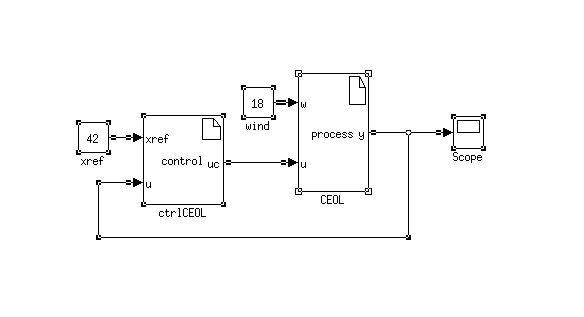
\includegraphics[scale=0.6]{eolcont.png}
\end{center}

Dove non viene rappresentato lo schema dell'errore ma una visione pi\'u reale del sistema
dove CEOL rappresenta il nostro rotore , e ctrlCEOL il controllo effettuato a monte del processo la cui uscita andr\'a a stimare il pitch delle pale.\\
Mentre xref il valore per cui si vuole che il rotore giri e in questo caso 42 RPM.
Andiamo a calcolare gli autovalori mediante il teorema dell'assegnazione degli autovalori.
\subsection{Assegnazione degli autovalori}
A questo punto per Ackermann abbiamo bisogno che la matrice di raggiungibilità abbia rango pieno, essendo quest'ultima 	il più grande sottospazio \\A-invariante contenuto nell'immagine di B.\\ \\
	Quindi:
	
\begin{equation*}
	\rho(\mathcal{R}):=
\rho(\:\begin{bmatrix}

	B&AB

\end{bmatrix}\:)=^{?}\rho_{max}=2
\end{equation*}

	Verifichiamo il tutto:
	
\begin{equation*}
\begin{bmatrix}

	B&AB

\end{bmatrix} =              %--------------uguale a-----------------
\begin{bmatrix}

	0&b\\b&ab

\end{bmatrix}
\end{equation*}

	Essendo $b=-2.8818$ abbiamo che il determinante della matrice  2x2 in esame risulta essere diverso da 0,
	e quindi il rango è pieno e pari a 2.\\
	Passiamo ad applicare la formula di Ackermann:
	
\begin{equation*}                    %----------Ackermann Formula------------
	K=
\begin{pmatrix}

	K_{1}&K_{2}

\end{pmatrix} =						%--------------uguale a----------------
\begin{pmatrix}

	K_{i}&K_{p}						

\end{pmatrix} = -					%--------------uguale a meno--------------
\begin{pmatrix}

	0&1						

\end{pmatrix}
\begin{pmatrix}

	B&AB					

\end{pmatrix}^{-1}p(A)
\end{equation*} \\

		Dove p(A) è il polinomio caratteristico p($\lambda$) desiderato con $\lambda=A$.\\\\
	In questo caso per assegnare due autovalori in -1 è stato scelto il seguente polinomio:\\

\begin{equation*}
	p(\lambda)_{des}=(\lambda+1)^{2}=\lambda^{2}+2\lambda+1        %---------------polinomio caratteristico------------
\end{equation*} \\
	
	ottenendo una matrice triangolare superiore
	
\begin{equation*}
	p(A)=A^{2}+2A+I_{2}=
\begin{pmatrix}

	1&a+2\\0&a^{2}+2a+1

\end{pmatrix}
\end{equation*} \\ \\

	La matrice dei coefficienti da trovare può ora essere calcolata come segue:

\begin{equation*}
	K=
\begin{pmatrix}

	K_{1}&K_{2}

\end{pmatrix} =                  %---------uguale a----------------
\begin{pmatrix}

	-\frac{1}{b}&0

\end{pmatrix}
\begin{pmatrix}

	1&a+2\\0&a^{2}+2a+1

\end{pmatrix} =                   %---------uguale a----------------
\begin{pmatrix}

	-\frac{1}{b}&-\frac{a+2}{b}

\end{pmatrix} =                    %---------uguale a----------------
\begin{pmatrix}

	K_{i}&K_{p}

\end{pmatrix} =                    %---------uguale a----------------
\begin{pmatrix}

	0.347&0.652

\end{pmatrix}
\end{equation*}\\

\subsection{Grafici sul controllo continuo}
Dai risultati, verifichiamo che i valori ottenuti rispecchino la teoria. \\
Per questo attraverso il Simnon \'e stato possibile implementare il sistema per valutarne i risultati mediante le simulazioni.
Nel seguente grafico viene mostrata la risposta del sistema per un ingresso di riferimento $u_r$=42 e
$\omega$=18, ovviamente essendo 42 il valore desiderato non terremo conto di $\omega$ ma bisogna comunque
tener presente che rappresentando la velocit\'a del vento ha un importante riscontro sulla dinamica del 
rotore.
\begin{center}
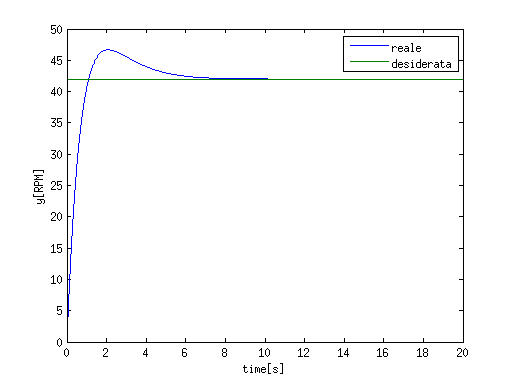
\includegraphics[scale=0.6]{graph/ycont.png}
\end{center}
Nel prossimo grafico invece andiamo ad esaminare l'azione controllante esercitata dal PI. 
\begin{center}
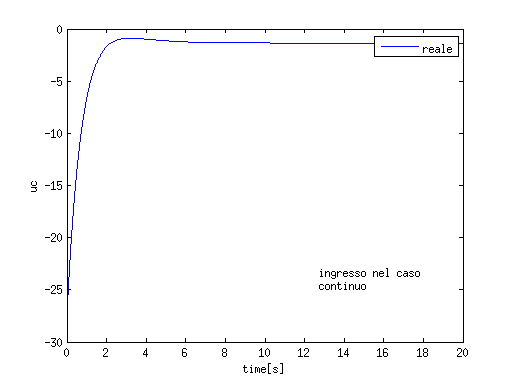
\includegraphics[scale=0.6]{graph/ucont.png}
\end{center}
	Qui di seguito sono stati inseriti due grafici nel caso in cui il segnale di velocità del vento sia di tipo 				sinusoidale. Il nostro controllo non prevede una gestione adatta al controllo di disturbi sinusoidali e, come si 			osserva a seguire, il valore picco picco dell'oscillazione si mantiene comunque vicino al valore desiderato pari a 42 		RPM. \\
\begin{center}
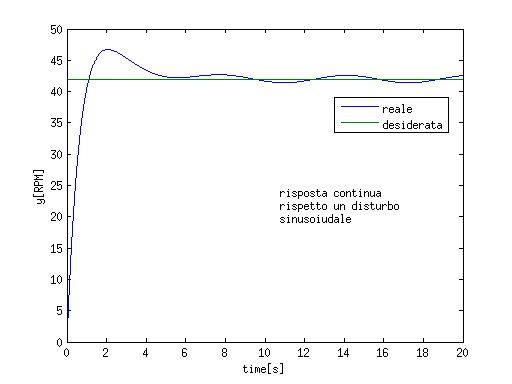
\includegraphics[scale=0.6]{graph/ycontsin.png}
\end{center}
	Notiamo nel grafico seguente che l'azione controllante nel caso di disturbo sinusoidale produce oscillazioni rispetto 		al valore medio osservato precedentemente nell'azione di controllo del PI.\\ Questi risultati verranno commentati 			anche nella sezione di controllo discreto, per una migliore visione d'insieme sui risultati ottenuti. \\
\begin{center}
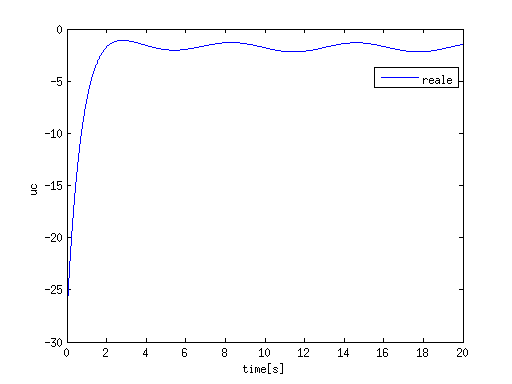
\includegraphics[scale=0.6]{graph/ucontsin.png}
\end{center}

Una volta constato che i valori calcolati per il controllo PI danno un ottima risposta 
da parte del sistema , siamo andati ad adattare il nostro sistema per effettuare un controllo digitale.\\
Non andremo direttamente a tradurre tutto il processo nell'ambito discreto ma faremo in modo che esso funzioni secondo tecniche di event-triggering.
%-------------Inizio parte discreta-----------------------

\section{Controllo discreto con Event Triggering}

	In questa parte parleremo del controllo discreto con ET della velocità di rotazione di una pala eolica mediante un
	controllore PI.\\ Qui di seguito lo schema di controllo, dove possiamo notare le prime differenze dallo schema 				precedente.
	
\begin{center}
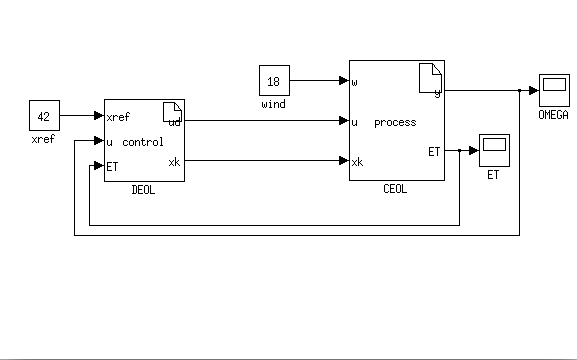
\includegraphics[scale=0.6]{eoltrig.png}
\end{center}

	Rispetto allo schema del controllo continuo osserviamo la presenza di un nuovo ramo diretto, dotato a sua volta di un
	feedback per la gestione dell'ET.\\ \\ \\ \\
	
\subsection{Ottimizzazione del criterio d'arresto}
	Un altro problema da affrontare è il calcolo della norma del prodotto PBK.
	Abbiamo bisogno di questo valore per gestire in maniera ottimale la soglia del criterio d'arresto nell'ET.\\
	Per ottenere il prodotto in esame, abbiamo bisogno della matrice P, soluzione dell'equazione di Sylvester, essendo già 	note le matrici B e K.\\ \\ \\ \\
	Ciò vale, tenendo conto della matrice dinamica $A_{c}$ :\\
	
\begin{equation*}
	A_{c}=A+BK=
\begin{pmatrix}

	0&1\\-0.0418&-2.9604

\end{pmatrix}
\end{equation*} \\
	
	Per risolvere l'equazione di Sylvester
	
\begin{equation*}
	A_{c}^{T}P + PA_{c} = -Q              %------------equazione di Sylvester----------------
\end{equation*}

	Scegliamo una matrice Q definita postiva, a piacere.\\
	Per le nostre simulazioni abbiamo utilizzato una matrice Q del tipo:\\

\begin{equation*}
	Q=
\begin{pmatrix}

	\frac{1}{2}&0\\0&657

\end{pmatrix}
\end{equation*}\\
	
	Ottenendo la matrice P dall'equazione di Sylvester mediante il MATLAB:\\
	
\begin{equation*}
	P=
\begin{pmatrix}

	22.4210&5.9774\\5.9774&112.9844

\end{pmatrix}
\end{equation*}\\

	E' possibile quindi calcolare il prodotto PBK ed applicarne la norma 2:\\
	
\begin{equation*}
	PBK=
\begin{pmatrix}

	-0.2500&-0.4697\\-4.7255&-8.8789

\end{pmatrix}
	\Rightarrow norm_{2}(PBK)=10.0722
\end{equation*}\\

	L'indice relativo al trigger, $\rho_{max}$ sarà dato infine da:
	
\begin{equation*}
	\rho_{max}=2\frac{\theta}{20.1443} \lambda_{min}^{Q}
\end{equation*}\\

	con $\lambda_{min}^{Q}$ autovalore minimo della matrice Q, ovvero pari a 0.5 .\\
	
	Il $\rho_{max}$ viene utilizzato come indice di peso per la commutazione del coefficiente dell'ET nel codice sorgente.
	\\ Il coefficiente dell'ET assumerà valore pari a 0, ovvero non agendo sul controllore, se il modulo dell'errore        	$n_{e}$ si mantiene sotto una certa soglia, definita proprio da:
	
\begin{equation*}
	n_{r}=\rho_{max}n_{x}
\end{equation*} \\

	con $n_{x}$ modulo dell'uscita.
	Altrimenti l'ET assume valore pari a 1, agendo sul sistema e quindi andando a stabilizzare il controllo.
	
\subsection{Grafici sul controllo discreto}
	
	Andiamo ora a discutere sui grafici ottenuti dal Simnon per quanto riguarda la simulazione nel tempo discreto.\\
	Osserviamo dal grafico seguente l'andamento del segnale d'uscita, e se lo confrontiamo con quello a tempo continuo, ci 	accorgiamo della bontà dell'azione dell'ET sul controllo del sistema, notando tutte le commutazioni che in uscita si 		traducono in una alternanza di valori che portano asintoticamente al valore desiderato di 42 RPM.
	
\begin{center}
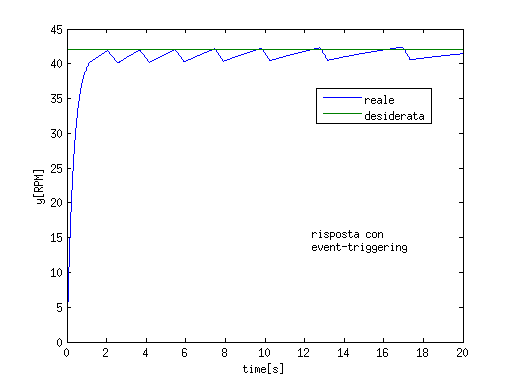
\includegraphics[scale=0.6]{graph/ydisc.png}
\end{center} 
	A seguire l'azione controllante a tempo discreto esercitata dal controllore PI. \\
	Notiamo inoltre l'azione dell'ET sul sistema osservando le continue commutazioni del segnale di controllo, assicurando 	stabilità al processo. E' presente inoltre un maggiore sforzo di controllo da parte del trigger fino ai 6 secondi, 			dovendo assestare con maggiore frequenza il contributo iniziale dell'uscita. \\ \\ 
\begin{center}
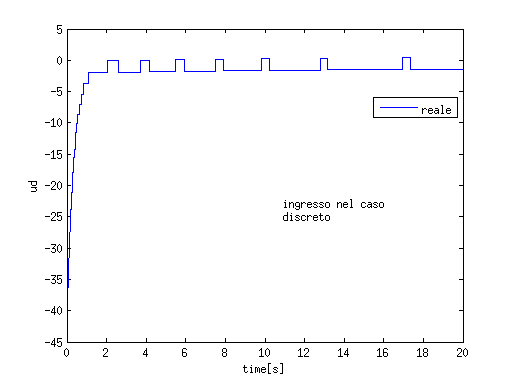
\includegraphics[scale=0.6]{graph/udisc.png} 
\end{center}
	Di seguito troviamo gli istanti di tempo in cui l'ET va ad agire sul controllo a tempo discreto.\\
\begin{center}
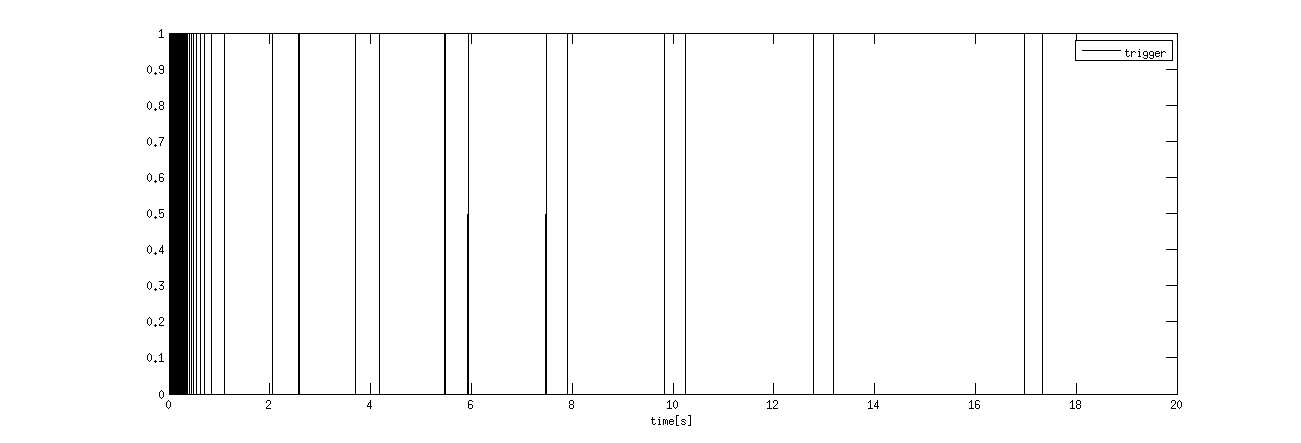
\includegraphics[scale=0.4]{graph/trigger1.png}
\end{center}
	La frequenza all'inizio è maggiore come illustrato precedentemente, fino ad assestarsi in corrispondenza del valore 		d'uscita desiderato.\\
	Nel caso invece di segnale di velocità del vento di tipo sinusoidale, nel tempo discreto abbiamo un margine 				d'affidabilità peggiore rispetto al caso continuo, avendo in uscita sempre delle commutazioni ma con valori non troppo 	vicini a quelli desiderati.
\begin{center}
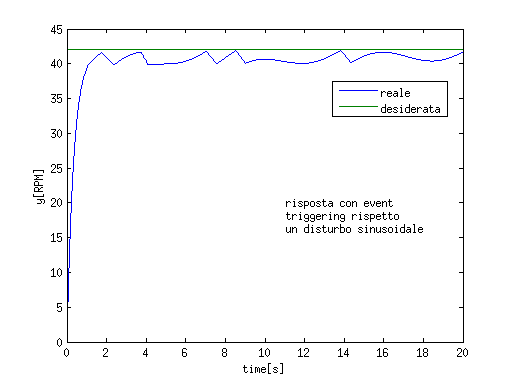
\includegraphics[scale=0.6]{graph/ydiscsin.png}
\end{center}
	Osserviamo nel grafico a seguire l'azione di controllo per disturbi sinusoidali.
\begin{center}
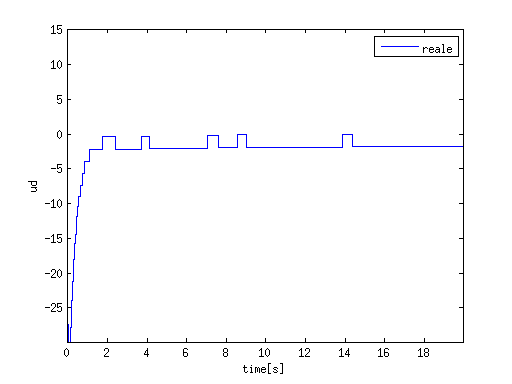
\includegraphics[scale=0.6]{graph/udiscsin.png}
\end{center}
	Nel grafico seguente le relative commutazioni del segnale di trigger.
\begin{center}
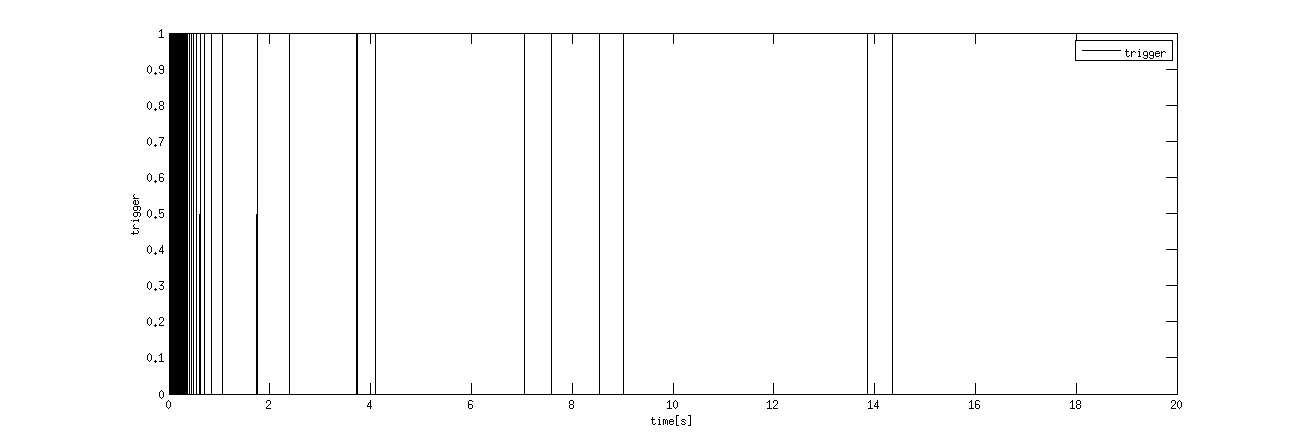
\includegraphics[scale=0.4]{graph/trigger2.png}
\end{center}



\end{document}


